%%%%%%%%%%%%%%%%%%%%%%%%%%%%%%%%%%%%%%%%%%%%%%%%%%%%%%%%%%%%
%%%%%%%%%%%%%%%%%%%%%%%%%%%%%%%%%%%%%%%%%%%%%%%%%%%%%%%%%%%%
%  Basic concepts in optimization and analysis
%%%%%%%%%%%%%%%%%%%%%%%%%%%%%%%%%%%%%%%%%%%%%%%%%%%%%%%%%%%%
%%%%%%%%%%%%%%%%%%%%%%%%%%%%%%%%%%%%%%%%%%%%%%%%%%%%%%%%%%%%
\chapter{
    %Basic concepts in optimization and analysis
    优化分析中的基本概念
    }  \label{chap:opt}
\chaptermark{Basic concepts}

\section{
    %Basic definitions and the notion of convexity
    凸性质的基本定义和概念
    }  \label{sec:optdefs}
\sectionmark{Basics}


%We consider minimization of a continuous function over a convex subset of Euclidean space. We mostly consider objective functions that are convex. In later chapters we relax this requirement and consider non-convex functions as well. 
考虑欧氏空间凸子集上连续函数的极小化问题,主要考虑凸的目标函数。
在后面的章节中,我们将放松这个要求,也考虑非凸函数。

%Henceforth,  let $\K \subseteq \reals^d$ be a bounded convex and compact set in Euclidean space. We denote by $D$ an upper bound on the diameter of $\K$:
因此,设 $\K \subseteq \reals^d$ 是欧几里德空间中的有界凸紧集。我们用 $D$ 表示直径 $\K$ 的上限: 
$$ \forall \x,\y \in \K , \ \|\x-\y\| \leq D.$$
%A set $\K$ is convex if for any  $\x,\y \in \K$, all the points on the line segment connecting $\x$ and $\y$ also belong to $\K$, i.e., 
如果对于任何 $\x, \y\ in \K$,连接 $\x$ 和 $\y$ 的线段上的所有点也属于$\K$,则集合 $\K$ 是凸的,也即, 
$$ \forall \alpha \in [0,1]  , \ \alpha \x + (1-\alpha)\y \in \K.$$
%A function $f: \K \mapsto \reals$ is convex if for  any $\x,\y \in \K$
如果对任意的 $\x,\y \in \K$ 有,
$$\forall \alpha \in [0,1] , \  f(  \alpha \x + (1-\alpha) \y) \leq  \alpha f(\x) + (1-\alpha) f(\y).$$
则函数  $f: \K \mapsto \reals$ 是凸的。

\paragraph{
    %Gradients and subgradients.
    梯度与次梯度。
    }
    
%The set of all subgradients of a function $f$ at $\x$, denoted $\partial f(\x)$, is the set of all vectors $\uv$ such that
 函数 $f$ 在 $\x$ 处的所有次梯度的集合,表示为 $\partial f(\x)$ ,是所有向量 $\uv$ 的集合,满足条件 
$$ f(\y) \geq  f(\x) + \uv^\top (\y-\x) . $$  
%It can be shown that the set of subgradients of a convex function is always non-empty. 
可以证明,凸函数的次梯度集总是非空的。 

%Suppose $f$ is differentiable, let $\nabla f(\x) [i] = \frac{\partial} {\partial \x_i} f(\x)$ be the vector of partial derivatives according to the variables, called the gradient. If the gradient $\nabla f(\x)$ exists, then $\nabla f(\x) \in \partial f(\x)$ and  $\forall \y \in \K$
假设 $f$ 是可微的,另 $\nabla f(\x) [i]=\frac{\partial}{\partial \x_i} f(\x)$ 是关于变量的偏导数向量,称为梯度。
如果梯度 $\nabla f(\x)$ 存在,那么 $\nabla f(\x) \ in\partial f(\x)$ 且 $\forall \y \in \K$
$$  f(\y) \geq f(\x) + \nabla f(\x)^\top (\y-\x).$$
%Henceforth we shall denote by $\nabla f(\x)$ the gradient, if it exists, or any member of $\partial f(\x)$ otherwise. 
因此,如果梯度存在,我们将用 $\nabla f(\x)$ 表示梯度,否则用 $\partial f(\x)$ 的任何成员表示梯度。 

%We denote by $G > 0$ an upper bound on the norm of the subgradients of $f$ over $\K$, i.e., $\|\nabla f(\x)\| \leq G$ for all $\x \in \K$. The existence of Such an upper bound implies that the function  $f$ is Lipschitz continuous with parameter $G$, that is, for all $\x,\y \in \K$
我们用 $G>0$ 表示 $f$ 在 $\K$ 上的次梯度范数的上界,即 $\|\nabla f(\x)\| \leq G$ 表示所有 $\x\in\K$。
这样一个上界的存在意味着函数 $f$ 与参数 $G$ 是 Lipschitz连续的,也就是说,对于所有 $\x, \y \in \K$ 有
$$ |f(\x) - f(\y)| \leq G \|\x-\y\|.$$


\paragraph{
    %Smoothness and strong convexity.
    平滑性和强凸性质。
    }

%The optimization and machine learning literature studies special types of convex functions that admit useful properties, which in turn allow for more efficient optimization. Notably, we say that a function is $\alpha$-strongly convex if
 优化和机器学习文献研究特殊类型的凸函数,这些凸函数具有有用的性质,从而实现更高效的优化。值得注意的是,我们称一个函数是 $\alpha$ 强凸的, 如果满足:
$$  f(  \y) \geq  f(\x) + \nabla f(\x)^\top (\y-\x)  + \frac{\alpha}{2} \|\y-\x\|^2.  $$
%A function is $\beta$-smooth if
一个函数是 $\beta$平滑的如果:
$$  f(  \y) \leq  f(\x) + \nabla f(\x)^\top (\y-\x)  + \frac{\beta}{2} \|\y-\x\|^2.  $$
%The latter condition is implied by a slightly stronger  Lipschitz condition over the gradients, which is sometimes used to defined smoothness, i.e., 
后一种条件可由梯度上稍强的Lipschitz条件得到,该条件有时用于定义平滑度,即:
$$ \| \nabla f(\x) - \nabla f(\y) \| \leq {\beta} \|\x-\y\|.$$

%If the function is twice differentiable and admits a second derivative, known as a Hessian for a function of several variables, the above conditions are equivalent to the following condition on the Hessian, denoted $\nabla^2 f(\x)$:
如果函数是二次可微的,并拥有一个二阶导数,也即多变量函数的 Hessian 矩阵,则上述条件等价于在 Hessian上满足以下条件,表示为 $\nabla^2 f(\x)$:
\begin{align*}
\text{
%Smoothness: 
平滑性:
}   \ \  -\beta  I \preccurlyeq &  \nabla^2 f(\x) \preccurlyeq \beta I \\
\text{
%Strong-convexity: 
强凸性:
}   \ \  \alpha  I \preccurlyeq  & \nabla^2 f(\x) ,
\end{align*}
%where $A\preccurlyeq B$ if the matrix $B-A$ is positive semidefinite.
其中,如果矩阵 $B-A$ 是半正定的,则 $A\preccurlyeq B$。 

%When the function $f$ is both $\alpha$-strongly convex and $\beta$-smooth, we say that it is $\gamma$-well-conditioned where $\gamma$ is the ratio between  strong convexity and smoothness, also called the {\it condition number} of $f$
当函数 $f$ 同时是 $\alpha$-强凸且 $\beta$-平滑时,我们说它是 $\gamma$-条件良好的,其中 $\gamma$ 是强凸和平滑之间的比率,也称为 $f$ 的{\it 条件数}。
$$ \gamma = \frac{\alpha}{\beta} \leq 1$$


\subsection{
    %Projections onto convex sets
    到凸集上的映射
    }  \label{sec:projections}
%In the following algorithms we shall make use of a projection operation onto a convex set, which is defined as the closest point inside the convex set to a given point. Formally,
在以下算法中,我们将使用凸集上的投影操作,凸集被定义为凸集内距离给定点最近的点。正式地
$$ \proj_\K (\y) \equaltri \argmin_{\x \in \K} \| \x - \y \|.$$
%When clear from the context, we shall remove the $\K$ subscript. It is left as an exercise to the reader to prove that the projection of a given point over a closed non-empty convex set exists and is unique. 
当从上下文中清除时,我们将删除 $\K$ 下标。留给读者一个练习:证明一个给定点在一个封闭的非空凸集上的投影是存在的,并且是唯一的。 

%The computational complexity of projections is a subtle issue that depends much on the characterization of $\K$ itself. Most generally, $\K$ can be represented by a membership oracle---an efficient procedure that is capable of deciding whether a given $\x$ belongs to $\K$ or not. In this case, projections can be computed in polynomial time. In certain special cases, projections can be computed very efficiently in near-linear time. 
投影的计算复杂性是一个微妙的问题,在很大程度上取决于 $\K$ 本身的特性。
大多数情况下,$\K$可以由成员关系先知表示(这是一个能够决定给定的$\x$是否属于$\K$ 高效的过程)。
在这种情况下,可以在多项式时间内计算出投影。
在某些特殊情况下,可以在近似线性时间内非常有效地计算投影。

%A crucial property of projections that we shall make extensive use of  is the Pythagorean theorem, which we state here for completeness:
我们将广泛使用的投影的一个关键特性是毕达哥拉斯定理,我们在这里说明它的完整性:
\begin{figure}[h!]
\begin{center}
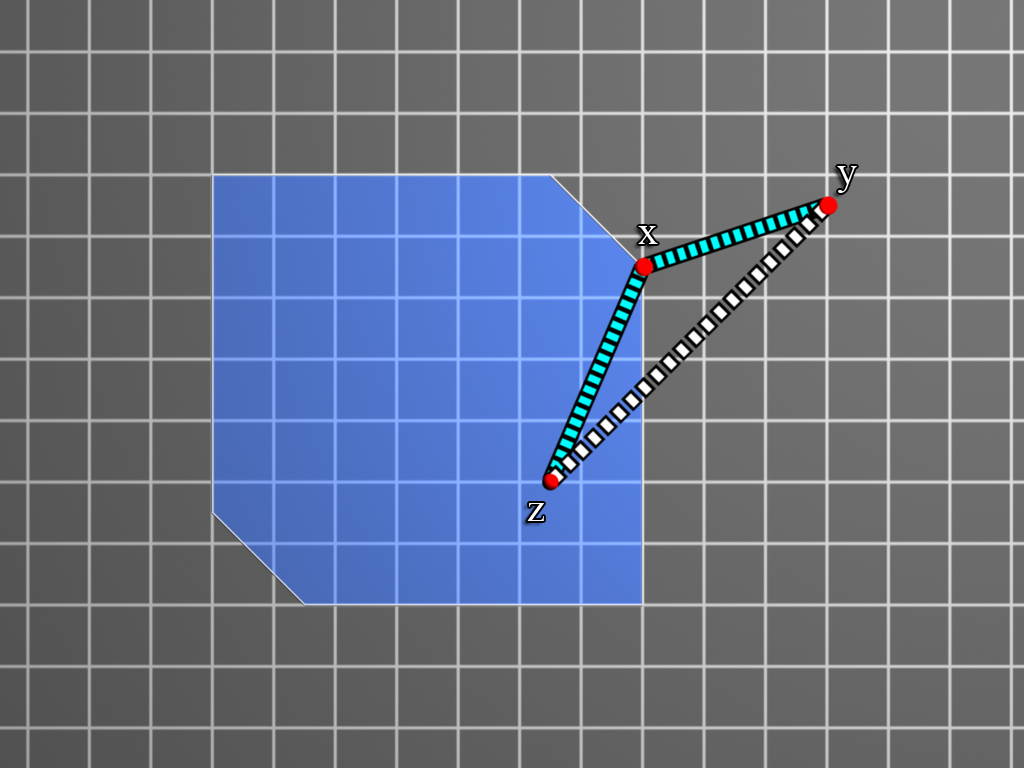
\includegraphics[width=3.5in]{figs/fig_pyth}%projection}
\end{center}
\caption{
    %Pythagorean theorem.
    毕达哥拉斯定理
    }
\end{figure}
\begin{theorem}[
    %Pythagoras, 	circa 500 BC
    毕达哥拉斯,约公元前500年
    ] \label{thm:pythagoras}
	%Let $\K \subseteq \reals^d$ be a convex set, $\y \in \reals^d$ and $\x = \proj_\K(\y)$. Then for any $\z \in \K$ we have
	令  $\K \subseteq \reals^d$ 是一个凸集合, $\y \in \reals^d$ 且 $\x = \proj_\K(\y)$。
    则 对于任意  $\z \in \K$ 我们有:
    $$ \| \y - \z \| \geq \| \x - \z \|.$$
\end{theorem}

%We note that there exists a more general version of the Pythagorean theorem. The above theorem and the definition of projections are true and valid not only for Euclidean norms, but for projections according to other distances that are not norms. In particular, an analogue of the Pythagorean theorem remains valid with respect to Bregman divergences. 
我们注意到毕达哥拉斯定理有一个更一般的版本。
上述定理和投影的定义不仅适用于欧几里德范数,而且适用于根据非范数的其他距离进行的投影。
特别是,毕达哥拉斯定理的类似物对于布雷格曼发散仍然有效。

\subsection{
    %Introduction to optimality conditions
    最优条件简介
    } 

%The standard curriculum of high school mathematics contains the basic facts concerning when a function (usually in one dimension) attains a local optimum or saddle point. The KKT (Karush-Kuhn-Tucker) conditions generalize these facts to more than one dimension, and the reader is referred to the bibliographic material at the end of this chapter for an in-depth rigorous discussion of optimality conditions in general mathematical programming. 
高中数学标准课程包含有关函数(通常为一维)何时达到局部最优或鞍点的基本事实。
KKT(Karush-Kuhn-Tucker)条件将这些事实推广到了不止一个维度,读者可以参考本章末尾的参考资料,深入、严谨地讨论一般数学规划中的最优条件。

%For our purposes, we describe only briefly and intuitively the main facts that we will require henceforth. We separate the discussion into convex and non-convex programming. 
出于我们的目的,我们只简单直观地描述了我们今后需要的主要事实。
我们将讨论分为凸规划和非凸规划。 

\subsubsection{
    %Optimality for convex optimization
    凸优化的最优性质
    } 

%A local minimum of a convex function is also a global minimum  (see exercises at the end of this chapter). 
%We say that $\x^\star$ is an $\epsilon$-approximate optimum if the following holds:
凸函数的局部极小值也是全局极小值(参见本章末尾的练习)。
我们说 $\x^\star$ 是一个 $\epsilon$ 近似最优值,如果以下条件成立:
$$ \forall \x \in \K \ . \  f(\x^\star) \leq f(\x) + \epsilon .$$ 
%It can be seen that a vanishing gradient implies $\epsilon$-optimality in bounded sets. 
可以看出,在有界集合中,消失梯度意味着 $\epsilon$-最优性。

%The generalization of the  fact that a minimum of a convex differentiable function on $\reals$ is a point in which its derivative is equal to zero, is given by the multi-dimensional analogue that its gradient is zero:
在 $\reals$ 上的凸可微函数的最小值是其导数等于零的点,对这一事实推广可以由其梯度为零的多维类比给出:
$$ \nabla f(\x ) =  0  \ \ \Longleftrightarrow  \ \ \x \in \argmin_{\x \in \reals^n} f(\x).$$ 


%We will require a slightly more general, but equally intuitive, fact for constrained optimization: at a minimum point of a constrained convex function, the inner product between the negative gradient and direction towards the interior of $\K$ is non-positive. This is depicted in Figure \ref{fig:optimality}, which shows that $-\nabla f(\x^\star)$ defines a supporting hyperplane to $\K$. The intuition is that if the inner product were positive, one could improve the objective by moving in the direction of the projected negative gradient. This fact is stated formally in the following theorem.
对于约束优化,我们需要一个更一般但同样直观的事实:在有约束凸函数的最小点,负梯度和朝向 $\K$内部的方向之间的内积是非正的。
这在图~\ref{fig:optimality}中描述,它显示了 $-\nabla f(\x^\star)$ 定义了一个支持 $\K$的超平面。
直觉是,如果内积是正的,可以通过向投影负梯度的方向移动来改善目标。
这一事实在下面的定理中有正式的表述。
\begin{theorem}[Karush-Kuhn-Tucker]  \label{thm:optim-conditions}
%Let $\K \subseteq \reals^d$ be a convex set, $\x^\star \in \argmin_{\x \in  \K} f(\x)$.  Then for any $\y \in \K$ we have
令 $\K \subseteq \reals^d$ 是一个凸集合,$\x^\star \in \argmin_{\x \in  \K} f(\x)$。则对于任意 $\y \in \K$ 我们有:
$$ \nabla f(\x^\star) ^\top ( \y - \x^\star ) \geq 0.  $$
\end{theorem}
\begin{figure}[h!]
\begin{center}
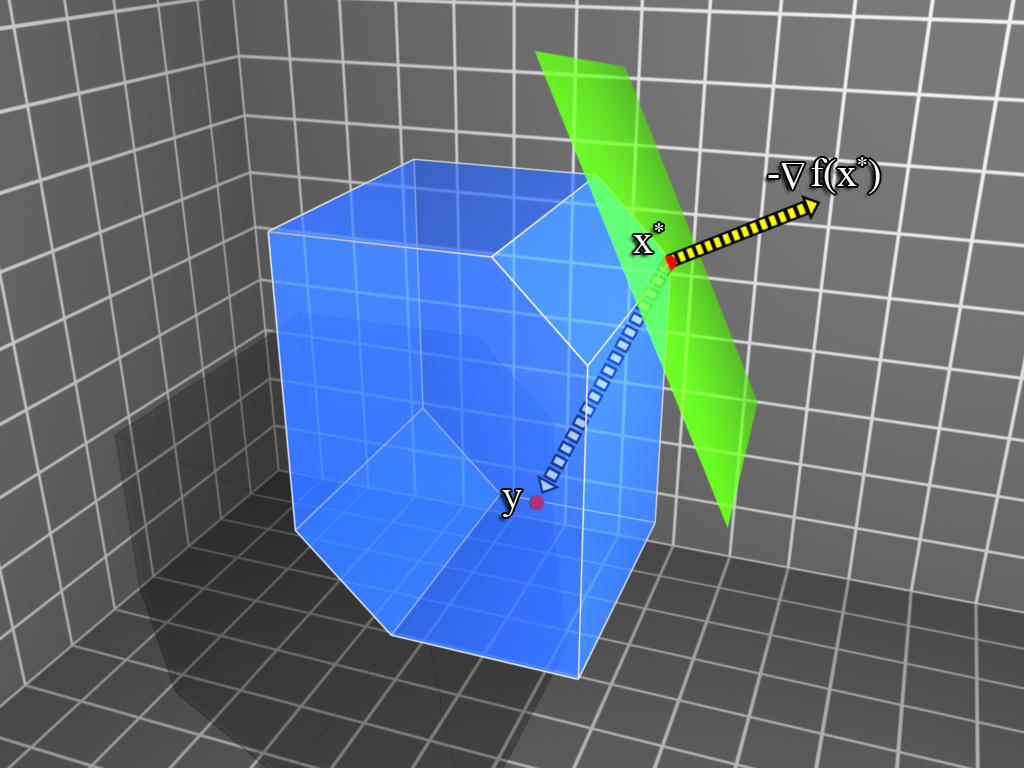
\includegraphics[width=4in]{figs/fig_kt}
\end{center}
\caption{
    %Optimality conditions: negative (sub)gradient pointing outwards. 
    最优条件:负(次)梯度指向外侧。
    \label{fig:optimality}}
\end{figure}


\subsection{
    %Solution concepts for non-convex optimization
    非凸优化的解的概念
    }

%We have seen in the previous chapter that mathematical optimization is NP-hard. This implies that finding global solutions for non-convex optimization is NP-hard, even for smooth functions over very simple convex domains. We thus consider other trackable concepts of solutions. 
我们在前一章中已经看到,数学优化是NP难的。
这意味着寻找非凸优化的全局解是NP困难的,即使对于非常简单的凸域上的光滑函数也是如此。
因此,我们考虑解决方案的其他可追踪概念。

%The most common solution concept is that of first-order optimality, a.k.a. saddle-points or stationary points. These are points that satisfy
最常见的解概念是一阶最优性,也就是鞍点或驻点。这些点满足如下条件:
$$  \| \nabla f(\x^\star ) \| = 0 . $$
%Unfortunately, even finding such stationary points is NP-hard.  We thus settle for approximate stationary points, which satisify
不幸的是,即使找到这样的静止点也是NP困难的。因此,我们满足于近似的静止点,满足:
$$  \| \nabla f(\x^\star ) \| \leq \epsilon . $$

\begin{figure}[h!]
\begin{center}
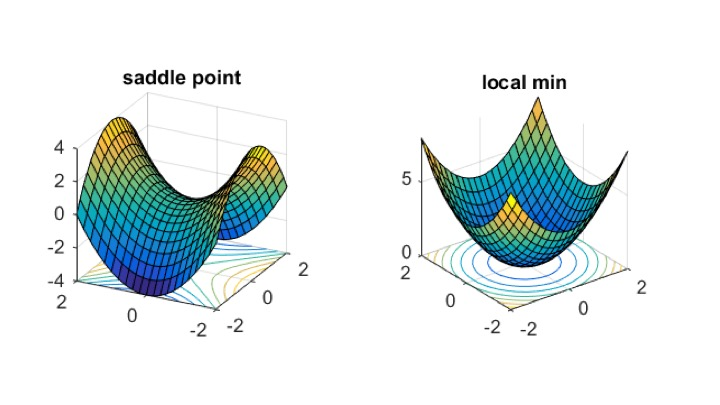
\includegraphics[width=3in]{./figs/optimums}
\end{center}
\caption{
%First and second-order local optima. 
一阶和二阶局部最优解。
\label{fig:optimums}}
\end{figure}

%A more stringent notion of optimality we may consider is obtained by looking at the second derivatives. We can require they behave as for global minimum, see figure \ref{fig:optimums}. Formally, we say that a point $\x^\star$ is a second-order local minimum if it satisfies the two conditions:
通过研究二阶导数,我们可以得到一个更严格的最优性概念。我们可以要求它们表现为全局最小值,参见图\ref{fig:optimums}。形式上,我们说点$\x^\star$是二阶局部极小值,如果它满足以下两个条件:
$$  \| \nabla f(\x^\star ) \| \leq \epsilon  \ , \   \nabla^2 f(\x^\star) \succeq -\sqrt{\eps} I . $$
%The differences in approximation criteria for first and second derivatives is natural, as we shall explore in non-convex approximation algorithms henceforth.
一阶导数和二阶导数的近似标准的差异是自然的,我们将在非凸近似算法中探讨这一点。

%We note that it is possible to further define optimality conditions for higher order derivatives, although this is less useful in the context of machine learning.  
我们注意到,可以进一步定义高阶导数的最优性条件,尽管这在机器学习环境中不太有用。

\section{
    %Potentials for distance to optimality
    距离最优性的可能性
    }

%When analyzing convergence of gradient methods, it is useful to use potential functions in lieu of function distance to optimality, such as gradient norm and/or Euclidean distance to optimality. The following relationships hold between these quantities. 
在分析梯度方法的收敛性时,使用势函数代替函数到最优性的距离是有用的,例如梯度范数和/或到最优性的欧氏距离。这些数量之间存在以下关系。

\begin{lemma} \label{lem:elementary_properties}
%The following properties hold for $\alpha$-strongly-convex functions and/or $\beta$-smooth functions over Euclidean space $\reals^d$. % over a constraint set $\K$: 
以下属性适用于欧氏空间 $\reals^d$上的 $\alpha$-强凸函数和/或 $\beta$-平滑函数。
\begin{enumerate}
    \item $\frac{\alpha}{2} d_t^2 \leq h_t$
    \item $ h_t \leq \frac{\beta}{2} d_t^2$
    \item $\frac{1}{2 \beta} \|\nabla_t\|^2 \leq h_t$
    \item $ h_t \leq \frac{1}{2 \alpha} \|\nabla_t\|^2 $
\end{enumerate}
\end{lemma}

\begin{proof}

\begin{enumerate}
\item  $h_t \geq \frac{\alpha}{2} d_t^2 $: %% case 1

%By strong convexity, we have 
根据强凸性质,我们有:
\begin{equation*}
\begin{array}{cl}
h_t & =  f(\x_t) - f(\x^{\star}) \\
& \geq  \nabla f(\x^{\star})^\top (\x_t - \x^{\star}) + \frac{\alpha}{2} \|\x_t - \x^{\star}\|^2  \\
 & = \frac{\alpha}{2} \|\x_t - \x^{\star}\|^2 
\end{array}
\end{equation*}
where the last inequality follows since the gradient at the global optimum is zero. 
其中,最后一个不等式成立是因为全局最优解处的梯度是 0。
    
    \item  $h_t \leq \frac{\beta}{2} d_t^2 $:  %% case 2
    
%By smoothness, 
根据平滑性质:
\begin{equation*}
\begin{array}{cl}
h_t & =  f(\x_t) - f(\x^{\star}) \\
& \leq  \nabla f(\x^{\star})^\top (\x_t - \x^{\star}) + \frac{\beta}{2} \|\x_t - \x^{\star}\|^2  \\
 & = \frac{\beta}{2} \|\x_t - \x^{\star}\|^2 
\end{array}
\end{equation*}
%where the last inequality follows since the gradient at the global optimum is zero. 
其中,最后一个不等式成立是因为全局最优解处的梯度是 0。



\item  $h_t \geq \frac{1}{2\beta} \|\nabla_t\|^2 $: % case 3
%Using smoothness, and let 
根据平滑性质,令
$\x_{t+1} = \x_t - \eta \nabla_t$ for $\eta = \frac{1}{\beta}$, 
\begin{equation*}
\begin{array}{cl}
h_t =  & f(\x_t) - f(\x^{\star}) \\
& \geq  f(\x_t) - f(\x_{t+1})   \\
 & \geq   \nabla f(\x_t)^\top (\x_{t} - \x_{t+1}) - \frac{\beta}{2} \|\x_t - \x_{t+1} \|^2   \\
 & = \eta \|\nabla_t\|^2  - \frac{\beta}{2} \eta^2 \|\nabla_t\|^2 \\
 & = \frac{1}{2\beta} \|\nabla_t\|^2  .
\end{array}
\end{equation*}



\item   $h_t \leq \frac{1}{2\alpha} \|\nabla_t\|^2 $:  %% case 3
    
%We have for any pair
对于任意的变量 对:
$\x,\y \in \reals^d$:
\begin{equation*}
\begin{array}{cl}
f(\y)  & \ge  f(\x) +   \nabla f(\x)^\top  (\y - \x ) + \frac{\alpha}{2}  \|\x - \y\|^2  \\
&\ge  \min_{\z \in \reals^d } \left\{ f(\x) +   \nabla f(\x)^\top  (\z - \x ) + \frac{\alpha}{2}  \|\x - \z\|^2 \right\} \\
& =  f(\x) - \frac{1}{2  \alpha} \| \nabla f(\x)\|^2. \\
& \text{ by taking $\z = \x - \frac{1}{ \alpha} \nabla f(\x) $ }
\end{array}
\end{equation*}
%In particular, taking 
特别的,取
$\x = \x_t \ , \ \y = \x^\star$, 
%we get
我们有
\begin{equation} \label{eqn:gradlowerbound}
 h_t =  f(\x_t) - f(\x^\star)  \leq \frac{1}{2 \alpha} \|\nabla_t\|^2  .
\end{equation}

\end{enumerate}
\end{proof}





\section{
    %Gradient descent and the Polyak stepsize
    梯度下降和Polyak步长
    } 

%The simplest iterative optimization algorithm is gradient descent, as given in Algorithm \ref{alg:basic}. We analyze GD with the Polyak stepsize, which has the advantage of not depending on the strong convexity and/or smoothness parameters of the objective function. 
最简单的迭代优化算法是梯度下降法,如算法\ref{alg:basic}中所示。我们用Polyak步长分析GD,它的优点是不依赖于目标函数的强凸性和/或光滑性参数。
\begin{algorithm}[h!]
\caption{
    %GD with the Polyak stepsize
    使用Polyak步长的GD
    }
\label{alg:basic}
\begin{algorithmic}[1]
\STATE Input: time horizon $T$, $x_0$
\FOR{$t = 0, \ldots, T-1$}
\STATE Set $\eta_t =  \frac{h_t}{\|\nabla_t\|^2} $
\STATE  $ \x_{t+1}  =   \x_t - \eta_t \nabla_t $
\ENDFOR
\STATE Return $\xbar = \argmin_{\x_t} \{ f(\x_t) \}$
\end{algorithmic}
\end{algorithm}


%To prove convergence bounds, assume $\|\nabla_t\| \leq G$, and define:
为了证明收敛界,假设 $\|\nabla_t\| \leq G$,并定义:
\begin{eqnarray*}
  B_T    &=&  \min\left\{
  \frac{G d_0}{\sqrt{ T}},
  \frac {2 \beta d_0^2}{ T },
  \frac{3 G^2}{  \alpha  T } ,
   \beta d_0^2\left(1-\frac{\alpha}{4\beta}\right)^T
 \right\}
\end{eqnarray*}

\begin{theorem} \label{thm:simple}
%(GD with the Polyak Step Size) 
(使用Polyak步长的GD)
%Algorithm \ref{alg:basic} attains the following regret bound after $T$ steps: 
算法 \ref{alg:basic} 在 $T$ 步数之后达到以下遗憾界限:
\begin{eqnarray*}
h(\xbar)  &=& \min_{ 0 \leq t \leq  T} \{ h_t \} \leq B_T % \\
\end{eqnarray*}
\end{theorem}




%Theorem~\ref{thm:simple} directly follows from the following lemma. Let $0\leq \gamma \leq 1 $,   define $R_{T,\gamma}$ as follows:
定理~\ref{thm:simple}直接来自下面的引理。让$0\leq\gamma\leq 1$定义$R{T\gamma}$,如下所示:
\[
  R_{T,\gamma} = \min\left\{
  \frac{G d_0}{\sqrt{\gamma T}},
  \frac {2 \beta d_0^2}{\gamma T },
  \frac{ 3 G^2}{{\gamma}  \alpha  T } ,
   \beta d_0^2\left(1-\gamma\frac{\alpha}{4 \beta}\right)^T
 \right\}
\, .
\]

\begin{lemma} \label{lemma:shalom2}
%For $0\leq \gamma \leq 1 $, suppose that a sequence $\x_0, \ldots \x_t$ satisfies:
对于 $0\leq \gamma \leq 1 $,假设有一个序列  $\x_0, \ldots \x_t$  满足:
\begin{equation} \label{eqn:shalom3}
d_{t+1}^2 \leq d_t^2 -  \gamma \frac{ h_t^2}{\|\nabla_t\|^2}
\end{equation}
%then for $\xbar$ as defined in the algorithm,
则,对于在算法中定义的 $\xbar$ 
 %$ = \argmin_{\x_t} \{ f(\x_t) \}$
%we have:
我们有
\[
h(\xbar)  \leq   R_{T,\gamma}\, .
\]
\end{lemma}



\begin{proof}
%The proof analyzes different cases:
本证明分析不同不同的情况:
\begin{enumerate}
\item
%For convex functions with gradient bounded by $G$, 
对于梯度由  $G$ 界定的凸函数:
\begin{eqnarray*}
d_{t+1}^2 -  d_t^2 & \leq - \frac{\gamma h_t^2}{\|\nabla_t\|^2} \leq -
                     \frac{\gamma h_t^2}{G^2}  
\end{eqnarray*}
%Summing up over $T$ iterations, and using Cauchy-Schwartz, we have
对 $T$次迭代相加求和,使用Cauchy Schwartz不等式,我们得到
\begin{eqnarray*}
\frac{1}{T} \sum_t h_t 
& \leq&  \frac{1}{\sqrt{T}} \sqrt{\sum_t h_t^2} \\
& \leq& \frac{ G}{\sqrt{\gamma T}} \sqrt{\sum_t (d_{t}^2 - d_{t+1}^2)} \leq
\frac{ G d_0 }{\sqrt{\gamma T}} \, .
\end{eqnarray*}

\item
%For smooth functions whose gradient is bounded by $G$,  Lemma~\ref{lem:elementary_properties} implies:
对于梯度由  $G$界定的平滑函数, Lemma~\ref{lem:elementary_properties} 意味着:
\[
d_{t+1}^2 - d_t^2 \leq - \frac{\gamma h_t^2}{\|\nabla_t\|^2} \leq -
\frac{\gamma h_t}{2 \beta} \, .
\]
%This implies
这意味着:
\[
\frac{1}{T} \sum_t h_t  \leq \frac{2 \beta d_0^2}{\gamma T}\, .
\]

\item
%For strongly convex functions, Lemma~\ref{lem:elementary_properties} implies:
对于强凸函数,Lemma~\ref{lem:elementary_properties} 意味着:
\[ d_{t+1}^2 - d_t^2
  \leq - \gamma \frac{h_t^2}{\|\nabla_t\|^2}
  \leq - \gamma \frac{h_t^2}{G^2}
  \leq  - \gamma  \frac{\alpha^2 d_t^4 }{4 G^2} \, .
\]
%In other words,
换句话说:
$d_{t+1}^2  \leq  d_t^2 ( 1- \gamma \frac{\alpha^2 d_t^2}{4 G^2} ) \, .$ 
%Defining $a_t :={\gamma}\frac{\alpha^2 d_t^2}{4 G^2}$, we have:
定义  $a_t :={\gamma}\frac{\alpha^2 d_t^2}{4 G^2}$ 我们有:
\[
a_{t+1}  \leq  a_t (1-a_t) \, .
\]
%This implies that $a_t \leq \frac{1}{t+1}$, which can be seen by induction
这意味着 $a_t\leq\frac{1}{t+1}$,这可以通过归纳法得到
\footnote{
%That $a_0\leq 1$ follows from Lemma \ref{lem:elementary_properties}. For $t=1$, $a_1\leq \frac{1}{2}$ since $a_1  \leq  a_0 (1-a_0)$ and $0\leq a_0\leq 1$.
$a_0\leq 1$ 可以由  Lemma \ref{lem:elementary_properties} 得到. 对于 $t=1$, $a_1\leq \frac{1}{2}$ 因为  $a_1  \leq  a_0 (1-a_0)$ and $0\leq a_0\leq 1$。
%For the induction step,
对于归纳步骤:
  $ a_t  \leq  a_{t-1} (1-a_{t-1}) \leq
  \frac{1}{t}(1-\frac{1}{t})
  =\frac{t-1}{t^2}=\frac{1}{t+1}(\frac{t^2-1}{t^2})
  \leq \frac{1}{t+1}$.}. 
%The proof is completed as follows\footnote{This assumes $T$ is even. $T$ odd leads to the same constants.} :  
证明完成如下 \footnote{假设$T$是偶数。$T$ 为奇数时也会带来相同的常数。}:
\begin{eqnarray*}
\frac{1}{ T/2 } \sum_{t= T/2 }^T h_t^2 &
\leq& \frac{2G^2}{\gamma  T  }\sum_{t= T/2 }^T ( d_t^2 -
                                   d_{t+1}^2)  \\
  &=&\frac{2 G^2}{\gamma  T } ( d _{ T/2 }^2 - d_T^2)  \\
  &=&\frac{8 G^4}{ \gamma^2 \alpha^2   T} ( a
    _{ T/2 } - a_T)  \\ 
   & \leq &\frac{9 G^4}{\gamma^2 \alpha^2 T ^2} 
  \, .
\end{eqnarray*}
%Thus, there exists a $t$ for which $h_t^2 \leq \frac{ 9 G^4}{\gamma^2 \alpha^2 T^2} $. Taking the square root completes the claim.
因此,存在一个  $t$ 使得  $h_t^2 \leq \frac{ 9 G^4}{\gamma^2 \alpha^2 T^2} $。求平方根就完成了证明。

\item
%For both strongly convex and smooth functions: 
对于同时强凸且平滑的函数:
\[ d_{t+1}^2 - d_t^2 \leq - \gamma \frac{h_t^2}{\|\nabla_t\|^2} \leq
 - \frac{\gamma h_t}{2 \beta} \leq
  - \gamma \frac{\alpha}{4\beta} d_t^2
  \]
  Thus,
  \[
    h_{T} \leq \beta d_{T}^2 \leq \beta d_0^2
    \left(1-\gamma\frac{\alpha}{4 \beta}\right)^T\, .
    \]
  \end{enumerate}
%This completes the proof of all cases.
如上完成所有情况的证明。
\end{proof}












\newpage
\section{
    %Exercises
    练习
    }


\begin{enumerate}

\item
%Write an explicit expression for the gradient and projection operation (if needed) for each of the example optimization problems in the first chapter. 
为第一章中的每个示例优化问题编写一个梯度和投影操作(如果需要)的显式表达式。

\item
%Prove that a differentiable function $f(x) : \mathbb{R} \rightarrow \mathbb{R}$ is convex if and only if for any $x,y\in\mathbb{R}$ it holds that $f(x)-f(y) \leq (x-y)f'(x)$.
证明可微函数 $f(x):\mathbb{R}\rightarrow\mathbb{R}$ 是凸的当且仅当对于任何 $x,y\in\mathbb{R}$ 它保持$f(x)-f(y) \leq(x-y)f'(x)$。

\item
%Recall that we say that a function $f:\mathbb{R}^n\rightarrow\mathbb{R}$ has a condition number $\gamma = \alpha/\beta$ over $K \subseteq \reals^d$ if the following two inequalities hold for all $\x,\y \in \K$:
回想一下,我们说过一个函数 $f:\mathbb{R}^n\rightarrow\mathbb{R}$ 有一个条件数$\gamma = \alpha/\beta$ 超过 $K \subseteq \reals^d$,如果以下两个不等式适用于所有$\x\y\in\K$:
\begin{enumerate}
\item $  f(\y) \geq f(\x) + (\y-\x)^{\top}\nabla{}f(\x) + \frac{\alpha}{2}\Vert{\x-\y}\Vert^2$
\item $  f(\y) \leq f(\x) + (\y-\x)^{\top}\nabla{}f(\x) + \frac{\beta}{2}\Vert{\x-\y}\Vert^2$
\end{enumerate}
%For matrices $A,B \in \reals^{n \times n}$ we denote $A \succcurlyeq B$ if $A-B$ is positive semidefinite. 
%Prove that if $f$ is twice differentiable and it holds that $\beta\textbf{I} \succcurlyeq \nabla^2f(\x) \succcurlyeq \alpha\textbf{I}$ for any $\x\in \K$, then the condition number of $f$ over $\K$  is $\alpha/\beta$.
对于矩阵 $A, B\in\reals^{n\times n}$,如果 $A-B$ 是半正定的,我们表示为 $A \succcurlyeq B$。
请证明,如果 $f$ 是两次可微的,并且对于任何 $\x\in\K$ 它保持 $\beta\textbf{I}\succcurlyeq\nabla^2f(\x) \succcurlyeq \alpha\textbf{I}$,那么 $f$超过 $\K$的条件数是$\alpha/\beta$。


\item
%Prove: 
证明:
\begin{enumerate}
	\item
	%The sum of convex functions is convex. 
    凸函数之和是凸函数。
	\item
	%Let $f$ be $\alpha_1$-strongly convex and $g$ be $\alpha_2$-strongly convex. Then $f+g$ is $(\alpha_1+\alpha_2)$-strongly convex. 
    设 $f$ 为 $\alpha_1$-强凸,$g$为 $\alpha_2$-强凸。那么 $f+g$是$(\alpha_1+\alpha_2)$-强凸的。
	\item
	%Let $f$ be $\beta_1$-smooth and $g$ be $\beta_2$-smooth. Then $f+g$ is $(\beta_1+\beta_2)$-smooth. 
    设 $f$ 为 $\beta_1$-平滑,$g$ 为 $\beta_2$-平滑。那么 $f+g$ 就是 $(\beta_1+\beta_2)$-平滑。
	
\end{enumerate}



\item
%Let $\K \subseteq \reals^d$ be closed, compact, non-empty and bounded. Prove that a necessary and sufficient condition for  $\proj_K(\x)$ to be a singleton, that is for $|\proj_K(\x)| = 1$, is for  $K$ to be  convex.
设 $\K\subseteq\reals^d$是封闭的、紧凑的、非空的和有界的。证明 $\proj_K(\x)$ 是一个单态(即 $\proj_K(\x)|=1$)的一个充要条件,是 $\K$是凸的。


\item
%Prove that for convex functions, $\nabla f(\x) \in \partial f(\x)$, that is, the gradient belongs to the subgradient set. 
证明对于凸函数,$\nabla f(\x)\in\partial f(\x)$, 即梯度属于次梯度集。

\item
 %Let $f(\x):\mathbb{R}^n\rightarrow\mathbb{R}$ be a convex differentiable function and $\K\subseteq \mathbb{R}^n$ be a convex set. Prove that $\x^\star\in \K$ is a minimizer of $f$ over $\K$ if and only if for any $\y\in \K$ it holds that $(\y-\x^\star)^{\top}\nabla f(\x^\star) \geq 0$.
 设 $f(\x): \mathbb{R}^n\rightarrow\mathbb{R}$ 为凸可微函数,$\K\subseteq\mathbb{R}^n$ 为凸集。证明 $\x^\star\in\K$ 是 $\K$上的 $f$的极小值,当且仅当对于任何$\y\in\K$它保持 $(\y-\x^\star)^{\top}\nabla f(\x^\star)\geq 0$。

\item
%Consider the $n$-dimensional simplex  $$\Delta_n = \lbrace{\x\in\mathbb{R}^n \, | \, \sum_{i=1}^n \x_i = 1, \, \x_i \geq 0 \ ,  \ \forall{i\in[n]}}\rbrace .$$
%Give an algorithm for computing the projection of a point $\x\in\mathbb{R}^n$ onto the set $\Delta_n$ (a near-linear time algorithm exists).
考虑一下$n$维单纯形
$$\Delta_n = \lbrace{\x\in\mathbb{R}^n \, | \, \sum_{i=1}^n \x_i = 1, \, \x_i \geq 0 \ ,  \ \forall{i\in[n]}}\rbrace .$$
给出一个算法来计算点 $\x\in\mathbb{R}^n$ 到集合 $\Delta_n$ 的投影(存在一个近似线性时间算法)。

\end{enumerate}





\newpage
\section{Bibliographic remarks}

%The reader is referred to dedicated books on convex optimization for much more in-depth treatment of the topics surveyed in this background chapter.  For background in convex analysis see the texts  \cite{borwein2006convex,rockafellar1997convex}. The classic textbook \cite{boyd.convex} gives a broad introduction to convex optimization with numerous applications. 
%For an adaptive analysis of gradient descent with the Polyak stepsize see \cite{hazan2019revisiting}.

读者可以参考关于凸优化的专门书籍,以更深入地处理本背景章节中调查的主题。有关凸分析的背景信息,请参阅文本 \cite{borwein2006convex,rockafellar1997convex}。经典教科书 \cite{boyd.convex}对凸优化进行了广泛的介绍,并给出了大量的应用。
有关Polyak步长梯度下降的自适应分析,请参见\cite{hazan2019revisiting}.